\documentclass[12pt,a4paper]{article}
\usepackage[latin1]{inputenc}
\usepackage{amsmath}
\usepackage{amsfonts}
\usepackage{amssymb}
\usepackage{natbib}
\usepackage{graphicx}
\usepackage{hyperref}
\graphicspath{ {images/} }

% Start of pseudo-code stuff
\usepackage{listings}
\usepackage{color}

\definecolor{dkgreen}{rgb}{0,0.6,0}
\definecolor{gray}{rgb}{0.5,0.5,0.5}
\definecolor{mauve}{rgb}{0.58,0,0.82}

\lstset{frame=tb,
  language=Java,
  aboveskip=3mm,
  belowskip=3mm,
  showstringspaces=false,
  columns=flexible,
  basicstyle={\small\ttfamily},
  numbers=none,
  numberstyle=\tiny\color{gray},
  keywordstyle=\color{blue},
  commentstyle=\color{dkgreen},
  stringstyle=\color{mauve},
  breaklines=true,
  breakatwhitespace=true,
  tabsize=3
} % End of pseudo-code stuff

\author{Roeland Krijgsman, Vince Vriend, Halat Naby}
\date{July 3rd, 2015}
\title{Python PageRank: relevantie van sites}

\begin{document}
\maketitle
\vspace{.5pc}
\centerline{\sc WISB256 - Programmeren in de Wiskunde}
\centerline{\it Vince Vriend (3894460), Roeland Krijgsman (3832171) en Halat Naby (3829030)}
\vspace{2pc}

\begin{abstract}
In deze opdracht word er een met behulp van python 3 een programma geconstrueerd dat het belang van een webpagina bepaald en dit kan ordenen.

Kernwoorden: Ordening, Belang, PageRank waarde, webpagina's.
\end{abstract}

\section{Inleiding}
PageRank is een methode die de belang van webpagina's ordent, waardoor het zoeken van data op het internet nauwkeuriger en doeltreffender kan gebeuren. De grondleggers van PageRank zijn de oprichters van Google Inc. Het eerste woord in PageRank refereert naar de Google-medeoprichter Larry Page en niet naar het woord pagina. PageRank is een continu proces dat dus up to date is. Het belang van een webpagina wordt bepaald door hoe vaak men verwijst naar een pagina en dit kan door PageRank aangeduid worden in een wiskundige PageRank-formule, zie hieronder. Er wordt een PageRank aangegeven bij een pagina die aangeeft hoe groot de kans eigenlijk is dat iemand op deze pagina terecht komt. PageRank geeft geen correlatie aan tussen de zoekwoorden die men gebruikt of de werkelijke inhoud van de sites. De PageRank van een pagina zal hoger worden wanneer er verwezen wordt naar andere links met hoge relevantie, maar dit ligt ook aan hoe groot de PageRank is van de pagina met de links erop. De links kunnen gezien worden als stemmen. Hoe meer stemmen, hoe belangrijker de gegeven site is. Hoe belangrijk een stem is, zal ook invloed hebben op de PageRank. 
\vspace{1pc}

Tegenwoordig is PageRank niet meer zo relevant. Dit komt omdat een site met een hogere PageRank niet hoger in de zoekresultaten te vinden zal zijn als men dit met een site met een lagere PageRank vergelijkt. Dit komt omdat er veel meer factoren binnen het algoritme aanwezig zijn, waarbij een zoekmachine zoals Google rekening mee houdt om webpagina's volledig te kunnen rangschikken op relevantie. De andere factoren houden ook rekening met de zoekwoorden en de inhoud van de sites. Hoewel het eigenlijk geen zin heeft om een hogere PageRank te behalen om hoger in de zoekresultaten voor te komen, geeft PageRank alsnog een zicht op de mate van belang van een pagina aan. Hiermee is het belangrijk dat je weet dat je PageRank in je achterhoofd moet houden, maar dat dit geen grote factor is die de relevantie van een site bepaalt in vergelijking met anderen. In dit verslag zal een programma ontwikkeld worden om het belang van een site te bepalen en hiervoor een PageRank te geven \cite{1} \cite{3}.

\section{Hoe bereken je een PageRank-waarde?}
Om een PageRank te bepalen voor een site, moet je ook de links die de pagina bevat mee moeten rekenen en de links buiten de site (bijvoorbeeld als men verwijst naar deze pagina). De wiskundige formule die helpt met de bepalen van de PageRank is als volgt: 
\[PR(A) = (1 - d) + d(\sum_{i=0}^{n}PR(T_{i})/C(T_{i}))\]
\begin{itemize}
\item $PR(A)$ = De PageRank van een pagina $x$
\item $C(x)$ = het totaal aantal uitgaande verwijzende links van pagina $x$
\item $\sum_{i=0}^{n}PR(T_{i})/C(T_{i})$ = de pagina's die verwijzen naar pagina $A$
\item $D$ = de dempingsfactor (tussen 0-1)
\end{itemize}

Uit deze formule kan de PR(A) de betekenis hebben dat het de kans aangeeft dat een wikkekeurig persoon op pagina A komt door op random verschillende links te drukken. Een andere betekenis kan bijvoorbeeld bepaling van de populariteit zijn van pagina A. 
\vspace{1pc}

Een lage waarde voor de dempingsfactor geeft aan dat de persoon die de pagina bezoekt snel zijn interesse verloren heeft en eindigt met het willekeurig aanklikken van de links.

Een hoge waarde (1 bijvoorbeeld) geeft dus het omgekeerde aan. De persoon op de pagina heeft meer interesse en zal langer willekeurige links aanklikken. De algemene waarde van d ligt vaak bij 0,85. 
\vspace{1pc}

Men kan de PageRank verhogen van A door andere pagina's die meer verwijzen naar de pagina a \cite{1}. De PageRank loopt van 0 tot 10. De sites met PageRank 0 zouden (zonder de andere factoren meegeteld die de zoekresultaat plaats bepalen) helemaal niet in de zoekresultaten moeten voorkomen, en een site met PageRank 10 zoals Google, Facebook en CNN zal boven aan moeten staan. Hieronder staat een figuur beschreven die de PageRank aangeeft van verschillende sites. Hoe hoger ``de berg", hoe meer inspanning het zal kosten. Een website hoort bij de ``Elite" als het een PageRank heeft tussen 8 en 10. \cite{3}

\vspace{1pc}
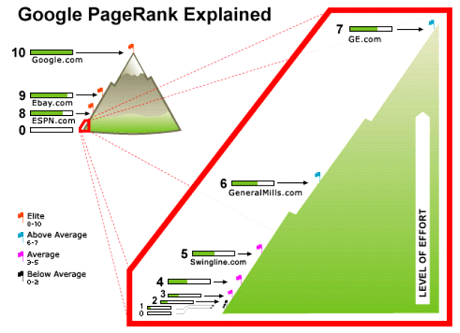
\includegraphics{GooglePageRankExplained}

Figuur 1. Uitleg over Pagerank \cite{2} 
\clearpage


\section{Hoe gaat het in zijn werk?}
De eerste stap is informatie van een document per link (document, pagina, webpage) bepalen:
\begin{itemize}
\item Titel van de pagina
\item URL
\item Hyperlink text waarmee verwezen wordt naar de pagina
\item Hyperlink text waarmee verwezen wordt naar andere pagina's
\item PageRank waarde
\end{itemize}

Hierna zal men informatie opzoeken per link:
\begin{itemize}
\item Site-informatie (Titel, URL)
\begin{itemize}
\item Bevat meestal de kern van de zaak, id's en onderwerp. Meer hebben we eigenlijk niet nodig, dus indexeren we niet de complete inhoud van de site. Dit zou namelijk ook meer schijfruimte en meer tijd kosten, en voegt niet voldoende toe om dit te verantwoorden
\item Op te slaan in een dictionary (zoekwoord, [URL])
\begin{itemize}
\item Te sorteren op PageRank
\end{itemize}
\end{itemize}
\item Links naar deze pagina
\item Links naar andere pagina's
\begin{itemize}
\item Ook binnen frames zoeken naar links
\item We negeren alles behalve php/html (dus geen plaatjes, scripts, opmaak, etc.)
\begin{itemize}
\item Links binnen plaatjes negeren vanwege advertenties etc. Hierbij accepteren we dat de gewone applicatie van plaatjes laten verwijzen naar pages binnen de site geen hogere PageRank geeft
\end{itemize} 
\end{itemize}
\clearpage
\item PageRank waarde
\begin{itemize}
\item We gebruiken de eenvoudige waarde, volgens de formule:
\[PR(A) = (1 - d) + d(\sum_{i=0}^{n}PR(T_{i})/C(T_{i}))\]
Wat we hier nog wel aan veranderen, is dat C(Ti) gelijk is aan nul, we deze pagina negeren.

d: vaak op 0.85 gezet, uit de paper van google over google pagerank. \cite{6}

Google itereert voor het hele internet 100 keer voor een goede schatting van de daadwerkelijke PageRank. Wij hoeven niet het hele internet te doen, maar willen wel graag een goede schatting - hiervoor hebben wij gekozen voor de waarde van 10
\end{itemize}
\end{itemize}

Vervolgens wordt er een datamodel geconstrueerd:
\begin{itemize}
\item URL Table
\begin{itemize}
\item n * 1, URL $\Rightarrow$ docID
\end{itemize}
\item DocID Table
\begin{itemize}
\item n * 1, docID $\Rightarrow$ URL
\end{itemize}
\item PageRank Table
\begin{itemize}
\item n * 1, docID $\Rightarrow$ PageRank
\item Wordt na iedere WebCrawl opnieuw gevuld
\end{itemize}
\item Reference Table
\begin{itemize}
\item n * n, docID $\Rightarrow$ docID
\item Wordt gevuld na de WebCrawl
\item Bevat 0/1 voor link van site met docID $\Rightarrow$ andere site met docID
\end{itemize}
\item Outgoing
\begin{itemize}
\item docID $\Rightarrow$ aantal
\end{itemize}
\item Incoming
\begin{itemize}
\item docID $\Rightarrow$ aantal
\end{itemize}
\item Webpages
\begin{itemize}
\item Webpage
\end{itemize}
\item Words
\begin{itemize}
\item word $\Rightarrow$ docID
\end{itemize}
\end{itemize}

GUI:
\begin{itemize}
\item Zoekplek
\begin{itemize}
\item Simple parsing
\begin{itemize}
\item Woord moet de goede letters bevatten, in volgorde (duplicates achter elkaar worden verwijderd)
\end{itemize}
\item Kan meerdere woorden zijn
\end{itemize}
\item Lijst met informatie van sites
\begin{itemize}
\item Geeft url + titel
\item Gesorteerd op PageRank
\end{itemize}
\end{itemize}

\begin{itemize}
\item Zoekt binnen 1 domein
\begin{itemize}
\item 1 WebCrawl inputfile voor het gekozen domein
\begin{itemize}
\item Dus: altijd een 100\% verbonden domein
\end{itemize}
\end{itemize}
\item Slaat op op schijf
\begin{itemize}
\item Wordt gebruikt voor PageRank
\end{itemize}
\end{itemize}

\section{Techniek}
We gebruiken vooral dictionaries en lists.
\subsection{Threading}
Een moderne desktop-processor voor consumenten heeft tegenwoordig minstens twee fysieke rekenkernen, ook wel ``cores" in het engels. Intel heeft ook nog een techniek genaamd hyperthreading waarbij een fysieke core zich aan het systeem presenteert als twee cores.
\clearpage

Vanuit het perspectief van de software zijn alle cores hetzelfde. Het zijn grofweg gezien individuele op zichzelf staande rekeneenheden die dus totaal onafhankelijk van elkaar rekenwerk kunnen verrichten. Dit betekent dat meerdere processen tegelijk kunnen werken. Je kan mail in je mail client ontvangen terwijl je met een browser op het internet surft. 
\vspace{1pc}

Binnen een proces kun je ook dingen tegelijk laten gebeuren. Dit gebeurt door in een proces een zogenaamde thread aan te laten maken. Een voorbeeld om dit nuttig toe te passen is bijvoorbeeld het optellen van veel getallen. Stel je hebt een rij van 1001 getallen waarvan je de totale som wilt weten. Je kan dit door een enkele rekenkern laten doen. Deze moet dan in zijn eentje 1000 optellingen doen om het antwoord te vinden.

Als we nu twee rekenkernen nemen en elk de helft van de rij laten optellen dan heb je 499 en 500 optellingen die tegelijk gebeuren en achteraf nog 1 optelling om de deelantwoorden op te tellen en het eindantwoord te vinden. In dit geval hebben we het probleem opgelost in de heflt van de tijd met techniek die praktisch iedereen in huis heeft.
\vspace{1pc}

Deze techniek werkt niet altijd. Wanneer je algoritme zeer sequentieel is waarbij elke volgende stap voortbouwt op het antwoord van de vorige stap kun je het probleem niet meer simpelweg in tweeen delen. Een voorbeeld hiervan is het toepassen van een hashfunctie op een waarde en weer een hashfunctie toepassen op het antwoord hiervan. Je kunt pas beginnen met stap twee wanneer stap 1 is afgelopen.
\vspace{1pc}

PageRank is wel uit te voeren op meerdere kernen tegelijk \cite{4}. Dit hebben wij niet gedaan in dit practicum. Toch hebben wij wel gebruik gemaakt van multithreading.
Ons zoekprogramma bestaat visueel uit een grafische interface. Deze voert constant de ``main loop" uit waardoor de interface steeds opnieuw getekend wordt en je dus visuele feedback krijgt op de interactie. Wanneer je een subtaak zoals de crawler of het PageRank algoritme zou starten binnen dezelfde thread als de main loop dan kan deze pas verder gaan nadat de subtaak klaar is. De crawler kan hele minuten in beslag nemen en dit zou de interface laten vastlopen voor de gebruiker.
Daarom starten wij de crawler en PageRank in een aparte thread zodat de gebruiker visuele feedback blijft krijgen over de voortgang van de subtaak door middel van een progress bar.

\section{Behaalde resultaten}
Ons programma is awesome. Zeker omdat de query ``advanced graphics" op \url{http://www.cs.uu.nl/education/} als eerste resultaat het vak ``Advanced Graphics" oplevert omdat deze het beste overeenkomt maar daarnaast ook de vakken ``Graphics" en ``Advanced Functional Programming".

\section{Mogelijke verbeteringen}
\subsection{Stemming}
Wanneer een gebruiker zoekt op de term ``auto" is het vaak ook relevant om resultaten van de zoekterm ``auto's" mee te nemen. Onze implementatie neemt zoektermen zeer letterlijk en kan deze stap zelf niet maken.
\vspace{1pc}

Er is wel een techniek voor, stemming \cite{5}.  Hiermee kun je vervoegingen van woorden terugbrengen naar de zogenaamde stamvorm. Bijvoorbeeld ``fishing", ``fished" en ``fisher" worden ``fish". In python kun je hier bijvoorbeeld de package PyStemmer voor gebruiken. Er zijn woordenboeken te downloaden zodat je niet zelf de complete taal hoeft uit te pluizen voor de mogelijke stamvorm van alle woorden. De woordenboeken zijn beschikbaar voor verschillende talen, ook Nederlands.
\vspace{1pc}

Hoewel wij geen stemming gebruiken is er wel aandacht besteed aan het organiseren van de zoekwoorden. Alle keywords worden in het programma eerst met de python casefold functie behandeld. Deze zorgt er niet alleen voor dat de string naar kleine letters wordt omgezet maar een ``{\ss}" wordt ook vervangen door ``ss" zodat gebruikers toch een beetje extra geholpen worden met het verkrijgen van het gewenste resultaat.

\section{Taakverdeling}
De taakverdeling is te vinden in Table 1: Taakverdeling.

\begin{table}
\caption{Taakverdeling}
\label{taakverdling}
\begin{center}
\begin{tabular}{|c||c|}
\hline
Taken: & Uitgevoerd door:\\
\hline
Het verslag & Halat Naby, Roeland Krijgsman, Vince Vriend\\
\hline
Het Algoritme &  Roeland Krijgsman en Vince Vriend\\
\hline
\end{tabular}
\end{center}
\end{table}

\bibliographystyle{plain}
\bibliography{paper}
\end{document}